\section{Heat Transfer Problem Example}

This example shows how to solve the problem using the Finite Element Method with a temperature-dependent thermal diffusivity. The considered geometry is an heterogeneous ellipsoid. The partial differential equation for transient heat transfer is:
$$ \rho c_p \dfrac{\partial T}{\partial t} = \nabla (\lambda \nabla T) $$
where $T$ is the temperature, $\rho$ is the material density, $c_p$ is the specific heat, and $\lambda$ is the thermal conductivity, among with the thermal diffusivity $\kappa = \frac{\lambda}{\rho c_p}$.\\

First, the ellipsoid geometry is defined : 

\begin{lstlisting}[language=Matlab]
nbr_cavities=5; 
geometry=tools.generateGeometry('ellipsoid',[1,0.5,0.5],nbr_cavities,'full',0.1,0.3);
geometry.exposed_faces=1;
\end{lstlisting}
\ 

Plot the geometry with cell labels displayed. These labels will be used to define heterogeneous material properties in the {\tt Simulate} function.

\begin{lstlisting}[language=Matlab]
figure;
pdegplot(geometry.structure, 'FaceAlpha', 0.2, 'CellLabels', 'on');
% delete axis
delete(findobj(gca,'type','Text')); 
delete(findobj(gca,'type','Quiver')); 
axis off; 
\end{lstlisting}

\begin{center}
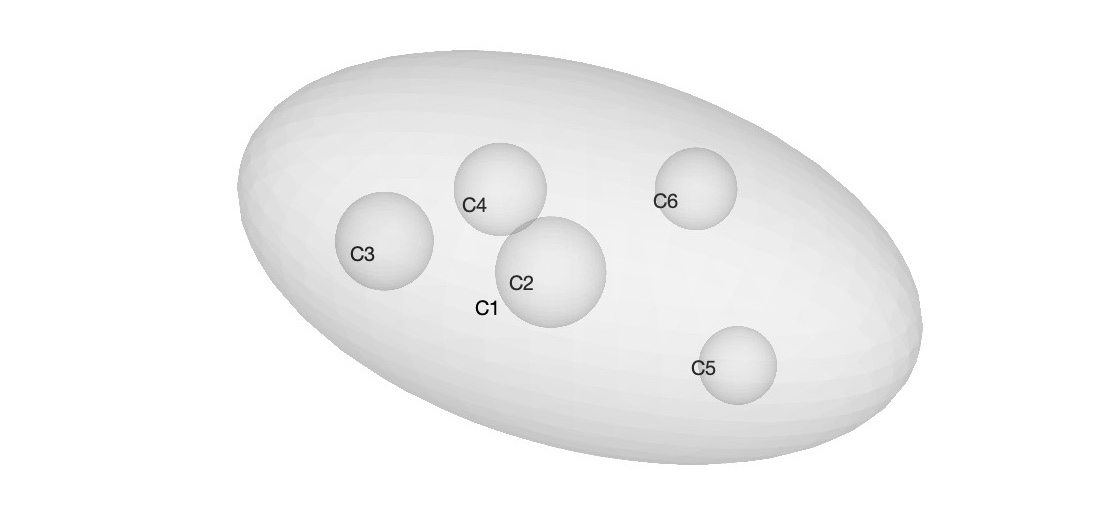
\includegraphics[scale=0.2]{Example/example_fig1.jpg}
\end{center}

Set properties of main material {\tt basalt} and heterogeneous material {\tt vaporised\_basalt}. 

\begin{lstlisting}[language=Matlab]
basalt.rho=1000;
basalt.cp=1000;
basalt.T_0=2000; 
basalt.lambda="tholeiitic";  % choose "tholeiitic", "dresser", "hebei"
vaporised_basalt.rho=1000;
vaporised_basalt.cp=1000;
vaporised_basalt.T_0=2000;
vaporised_basalt.lambda="hebei";  % choose "tholeiitic", "dresser", "hebei"
\end{lstlisting}
\

Set the parameters of the problem. 

\begin{lstlisting}[language=Matlab]
options.material=basalt;
options.cavities_material=vaporised_basalt;
options.latent_heat=0;        % (J/kg) Latent heat of basalt = 4e5. 
                              % Set to 0 for no-latent heat
options.T_latent=1373;        % (K) Crystallization temperature of basalt
options.eps=1;                % Emissivity
options.TCurie=858;           % (K) Curie temperature
options.T_out=300;            % (K) Outer space temperature
options.tmax=6*3600*24;       % (s) max integration time
options.dt=200;               % (s) time-step 
\end{lstlisting}
\

Call the {\tt simulate} function. A description of the implementation of the function can be found in the next section.

\begin{lstlisting}[language=Matlab]
simulation=Simulate(geometry, options);
\end{lstlisting}
\

One can get the coordinates and time when the whole geometry reached the Curie temperature, to plot the thermal evolution over time at that node, using the built-in PDE function {\tt interpolateTemperature}.

\begin{lstlisting}[language=Matlab]
Result=tools.getThermalBarycenter(simulation, options.TCurie);
tempBar=interpolateTemperature(simulation,Result.Bar,1:numel(simulation.SolutionTimes));
figure; 
plot(simulation.SolutionTimes, tempBar, '-b');
xlabel('t (days)');
ylabel('T (K)');
title('Thermal evolution at last point reaching Curie temperature');
grid on; 
\end{lstlisting}

\begin{center}
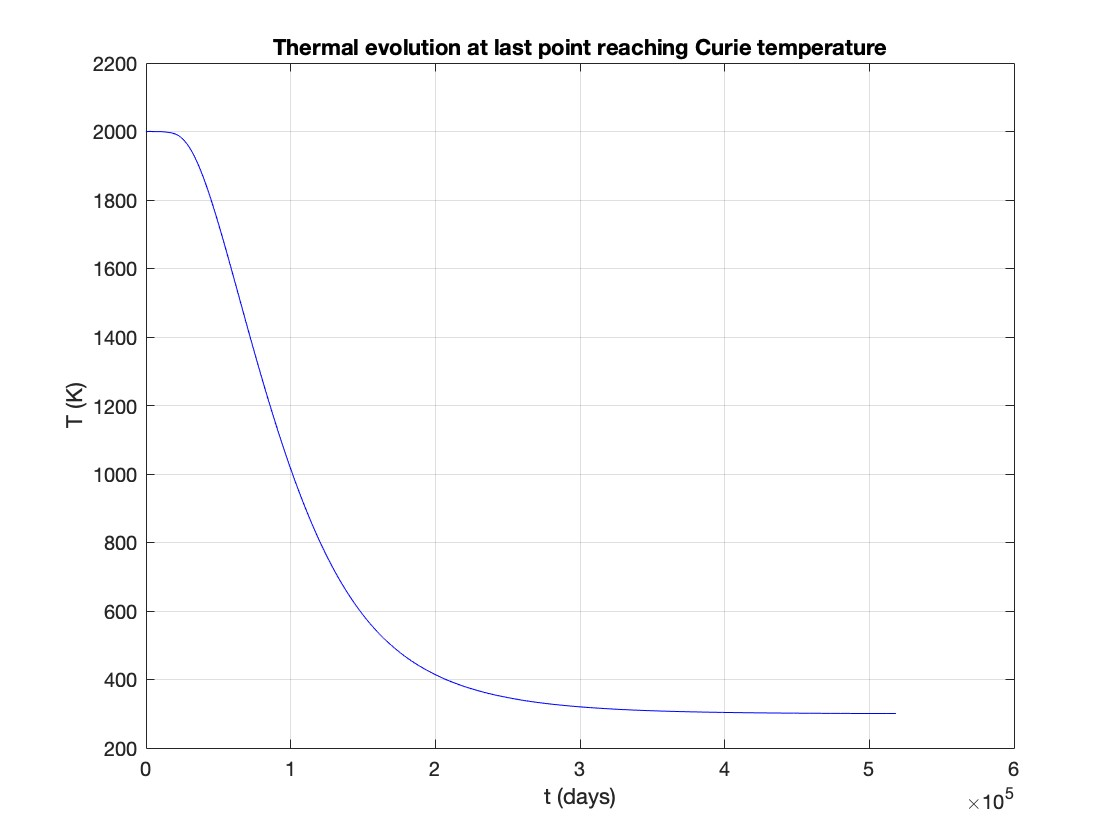
\includegraphics[scale=0.25]{Example/example_fig2.jpg}
\end{center}



All the results of the simulation can be saved in a structure and in a file

\begin{lstlisting}[language=Matlab]
results.simulation=simulation;
results.temperature = simulation.Temperature;
results.nodes = simulation.Mesh.Nodes;
results.tlist=simulation.SolutionTimes;
results.tempBar=tempBar;
results.bar=Result.Bar;
results.time=Result.Time/(3600*24);
results.nbr_cavities=geometry.nbr_cavities;
results.volume=geometry.volume;
results.porous_volume=geometry.porous_volume;
results.porosity_fraction=(results.porous_volume/results.volume)*100;
\end{lstlisting}
\

Results can now be used to plot animations or figures. 

\begin{lstlisting}[language=Matlab]
tools.geometryView('Geometry.pdf', simulation, geometry);
tools.isosurface('Animation.avi', simulation, options.TCurie);
tools.heatMapSlice('Slice.pdf',simulation,'z',0);
tools.heatMapSliceAnimation('SliceVideo.avi',simulation,'z',0);
\end{lstlisting}

\medskip
Results can also be extracted to use in \textsc{Python} thanks to the {\tt getPythonResults} from the {\tt .mat} file.